\chapter{遗传变异与疾病}\label{ch:g11:genes-and-disease}

一对身体健康的夫妇有了第一个孩子，这孩子从
出生最初几周起便咳嗽、体重不增，汗液咸得
连额头上的一吻都能尝出咸味。诊断为囊性纤维化：
夫妇双方在不知情的情况下，各自携带了同一\omterm{def:g10:universal-dna:gene}{基因}的一个失效拷贝，
孩子则同时继承了两个。欧洲血统人群中每 25 人便有 1 人
是这样的携带者；这对夫妇本可在怀孕前
通过一滴血的检测得知。本章
讨论的是写在\omterm{def:g10:universal-dna:gene}{等位基因}中的疾病：它们如何遗传，
如何由家系图计算风险，实验室如何读取
\omterm{def:g10:universal-dna:gene}{基因}，以及大多数常见病为何只是部分由遗传决定。

\section{单基因疾病}

\begin{definition}[遗传病、显性与隐性]\label{def:g11:genes-and-disease:genetic}
若某疾病由一个或多个\omterm{def:g11:mutations:mutation}{突变}\omterm{def:g10:universal-dna:gene}{等位基因}引起，则称之为\emph{遗传病}\index{遗传病}。
对于单\omterm{def:g10:universal-dna:gene}{基因}疾病，某\omterm{def:g10:universal-dna:gene}{等位基因}若仅在携带两个该拷贝的人身上
才表现出疾病，则称之为\emph{隐性}\index{隐性}的；
仅携带一个拷贝的人是健康的
\emph{携带者}\index{携带者}；若一个拷贝即足以致病，则称之为\emph{显性}\index{显性}的。
按惯例，同一\omterm{def:g10:universal-dna:gene}{基因}的\omterm{def:g10:universal-dna:gene}{等位基因}用字母表示：
正常\omterm{def:g10:universal-dna:gene}{等位基因}记为 $A$，隐性\omterm{def:g11:mutations:mutation}{突变}\omterm{def:g10:universal-dna:gene}{等位基因}记为 $a$，
因此携带者为 $Aa$，患者为 $aa$。
\end{definition}

\begin{example}[囊性纤维化]\label{ex:g11:genes-and-disease:cf}
CFTR \omterm{def:g10:universal-dna:gene}{基因}编码一种\omterm{def:g11:gene-expression:protein}{蛋白质}，它使氯离子穿过
衬于气道、肠道与汗腺的\omterm{def:g10:cells-common-unit:cell}{细胞}膜，
最常见的\omterm{def:g11:mutations:mutation}{突变}\omterm{def:g10:universal-dna:gene}{等位基因}缺失三个\omterm{def:g10:universal-dna:nucleotide}{核苷酸}，因而少了一个
\omterm{def:g10:chemistry-of-life:families}{氨基酸}；该\omterm{def:g11:gene-expression:protein}{蛋白质}错误折叠并被降解。失去它后，
气道的黏液变得黏稠，感染在
肺部滞留，胰腺导管堵塞。该病为\omterm{def:g11:genes-and-disease:genetic}{隐性}遗传：欧洲人中约
每 25 人有 1 人为健康携带者，每 2500 名新生儿中有 1 人
患病。镰状\omterm{def:g10:cells-common-unit:cell}{细胞}病（\cref{ch:g11:enzymes-and-phenotype}）
同样为\omterm{def:g11:genes-and-disease:genetic}{隐性}遗传；亨廷顿病是脑部的退行性变化，
约四十岁起病，为\omterm{def:g11:genes-and-disease:genetic}{显性}遗传——一个\omterm{def:g11:mutations:mutation}{突变}\omterm{def:g10:universal-dna:gene}{等位基因}
即已足够，每位患者都有一位患病的亲代。
\end{example}

\begin{proposition}[隐性遗传病的传递]\label{prop:g11:genes-and-disease:recessive}
每位亲代随机将其两个\omterm{def:g10:universal-dna:gene}{等位基因}中的一个传给每个孩子。
因此，两个携带者 $Aa \times Aa$ 的每个孩子
为患病者的概率为 $1/4$（$aa$），为携带者的概率为 $1/2$（$Aa$），
为非携带者的概率为 $1/4$（$AA$）。携带者与非携带者
$Aa \times AA$ 的子代无人患病，每个孩子为携带者的
概率为二分之一。患病者与非携带者 $aa \times AA$ 的子代
全部为携带者。
\end{proposition}
\admitted

\begin{omfigure}
\begin{tikzpicture}[font=\small]
  \draw[thick] (0,0) grid[step=1.6] (3.2,3.2);
  \node[anchor=south] at (0.8,3.3) {$A$}; \node[anchor=south] at (2.4,3.3) {$A$};
  \node[anchor=east] at (-0.15,2.4) {$A$}; \node[anchor=east] at (-0.15,0.8) {$a$};
  \node[anchor=south, font=\small\itshape] at (1.6,3.75) {父亲的等位基因};
  \node[anchor=east, font=\small\itshape, rotate=90] at (-0.65,1.6) {};
  \node[font=\small\itshape, rotate=90, anchor=south] at (-0.75,1.6) {母亲的等位基因};
  \node[fill=omDef!15, minimum size=1.5cm] at (0.8,2.4) {$AA$};
  \node[fill=omDef!15, minimum size=1.5cm] at (2.4,2.4) {$AA$};
  \node[fill=omProp!20, minimum size=1.5cm] at (0.8,0.8) {$Aa$};
  \node[fill=omProp!20, minimum size=1.5cm] at (2.4,0.8) {$Aa$};
  \node[anchor=north, align=center] at (1.6,-0.3) {携带者母亲 $\times$ 非携带者父亲：\\ 一半子女为携带者，无人患病};
  \begin{scope}[xshift=9.6cm]
    \draw[thick] (0,0) grid[step=1.6] (3.2,3.2);
    \node[anchor=south] at (0.8,3.3) {$A$}; \node[anchor=south] at (2.4,3.3) {$a$};
    \node[anchor=east] at (-0.15,2.4) {$A$}; \node[anchor=east] at (-0.15,0.8) {$a$};
    \node[fill=omDef!15, minimum size=1.5cm] at (0.8,2.4) {$AA$};
    \node[fill=omProp!20, minimum size=1.5cm] at (2.4,2.4) {$Aa$};
    \node[fill=omProp!20, minimum size=1.5cm] at (0.8,0.8) {$Aa$};
    \node[fill=omThm!25, minimum size=1.5cm] at (2.4,0.8) {$aa$};
    \node[anchor=north, align=center] at (1.6,-0.3) {双方均为携带者：$1/4$ 患病，\\ $1/2$ 为携带者，$1/4$ 为非携带者};
  \end{scope}
\end{tikzpicture}

{\small 棋盘方格（庞纳特方格）。每个格子是一种等可能的组合：母亲的\omterm{def:g10:universal-dna:gene}{等位基因}（行）
与父亲的\omterm{def:g10:universal-dna:gene}{等位基因}（列）组合而成。图中比例
是每个孩子的概率，而非对四个孩子的保证。}
\end{omfigure}

\begin{omfigure}
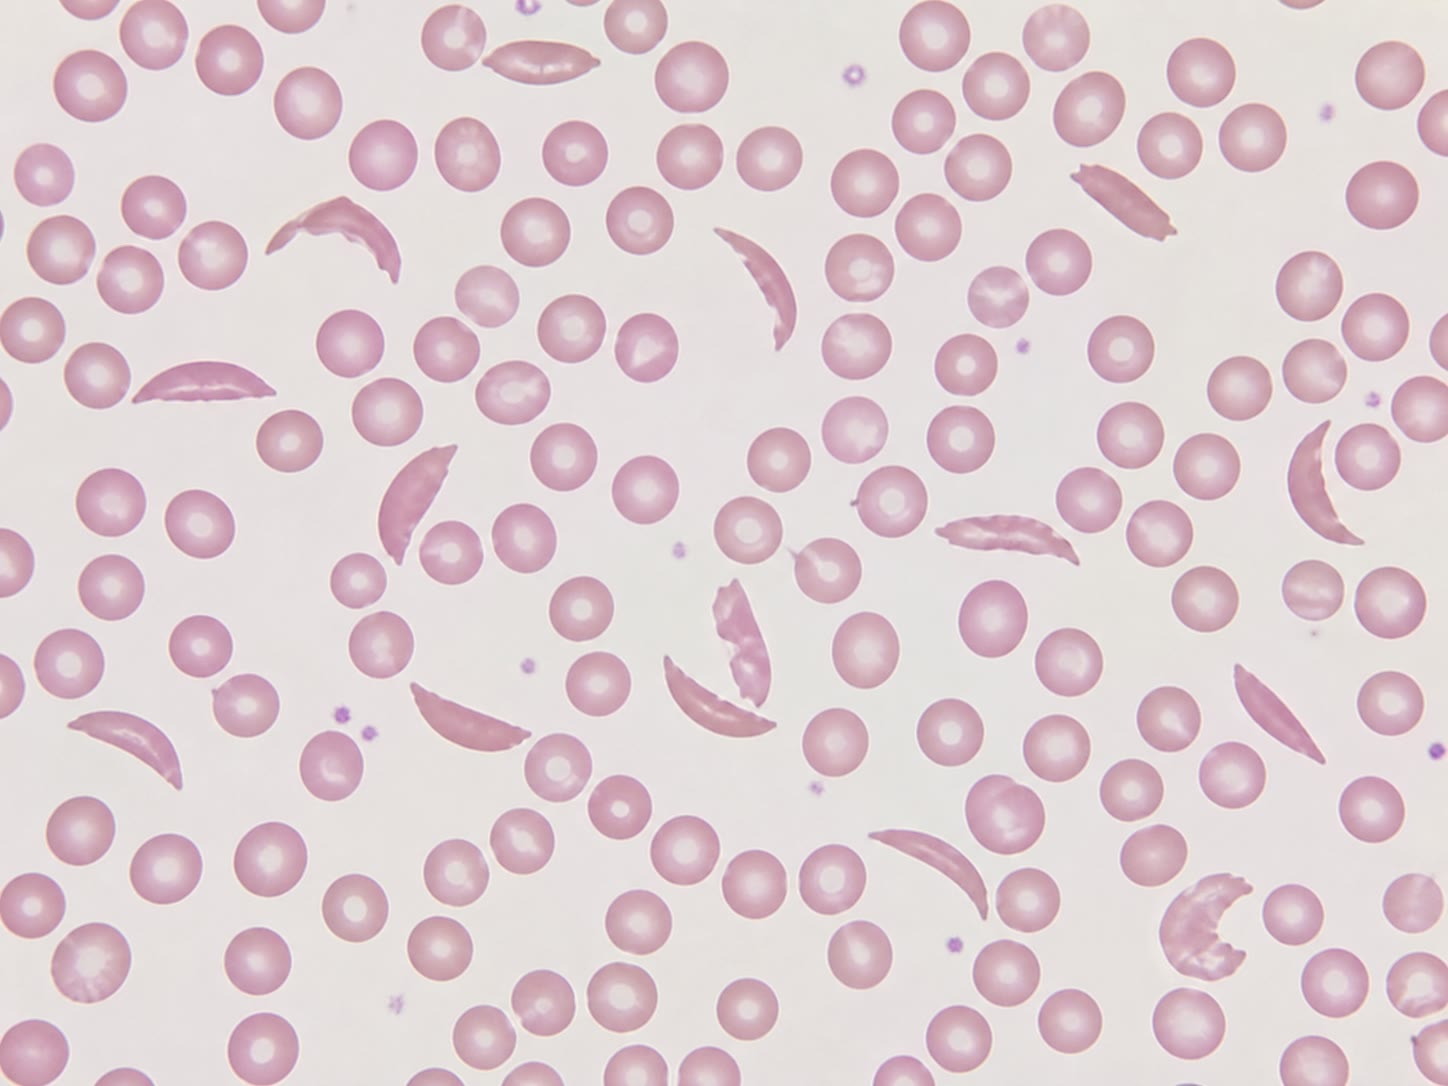
\includegraphics[width=0.56\linewidth]{images/book2/ai/g11-disease-sickle-smear.jpg}

{\small 镰状\omterm{def:g10:cells-common-unit:cell}{细胞}病患者的血涂片：圆形
红\omterm{def:g10:cells-common-unit:cell}{细胞}，其中夹有镰刀形\omterm{def:g10:cells-common-unit:cell}{细胞}。这是一个\omterm{def:g10:chemistry-of-life:families}{氨基酸}
替换在两个\omterm{def:g10:universal-dna:gene}{等位基因}上均存在时所呈现的\omterm{def:g10:cells-common-unit:cell}{细胞}水平\omterm{def:g11:enzymes-and-phenotype:phenotype}{表型}。}
\end{omfigure}

\section{读懂家系图}

\begin{definition}[系谱图]\label{def:g11:genes-and-disease:pedigree}
\emph{系谱图}\index{系谱图}是表示一个家族跨越数代的图示：
用方框表示男性，圆圈表示女性，
用横线连接一对配偶，用竖线连向其子女，
用实心符号表示患病者。世代自上而下依次用 I、II、III 编号，
同一代中个体从左到右编号。
\end{definition}

\begin{omfigure}
\begin{tikzpicture}[font=\small, line cap=round]
  \tikzset{m/.style={draw, thick, minimum size=0.5cm, inner sep=0},
           f/.style={draw, thick, circle, minimum size=0.5cm, inner sep=0},
           aff/.style={fill=omThm!70}}
  % generation I
  \node[m] (I1) at (2,3) {}; \node[f] (I2) at (3.2,3) {};
  \node[m] (I3) at (6.4,3) {}; \node[f] (I4) at (7.6,3) {};
  \draw[thick] (I1) -- (I2); \draw[thick] (I3) -- (I4);
  \node[anchor=east] at (0.8,3) {I};
  \foreach \n/\x in {1/2, 2/3.2, 3/6.4, 4/7.6} \node[font=\scriptsize, anchor=south] at (\x,3.35) {\n};
  % generation II
  \draw[thick] (2.6,3) -- (2.6,2.3) -- (4.4,2.3); \draw[thick] (1.6,2.3) -- (2.6,2.3);
  \draw[thick] (7.0,3) -- (7.0,2.3) -- (5.6,2.3); \draw[thick] (7.0,2.3) -- (8.4,2.3);
  \node[f] (II1) at (1.6,1.7) {}; \node[m, aff] (II2) at (2.6,1.7) {}; \node[m] (II3) at (4.4,1.7) {};
  \node[f] (II4) at (5.6,1.7) {}; \node[f] (II5) at (7.0,1.7) {}; \node[m] (II6) at (8.4,1.7) {};
  \foreach \x in {1.6,2.6,4.4,5.6,7.0,8.4} \draw[thick] (\x,2.3) -- (\x,1.95);
  \draw[thick] (II3) -- (II4);
  \node[anchor=east] at (0.8,1.7) {II};
  \foreach \n/\x in {1/1.6, 2/2.6, 3/4.4, 4/5.6, 5/7.0, 6/8.4} \node[font=\scriptsize, anchor=north] at (\x,1.42) {\n};
  % generation III
  \draw[thick] (5.0,1.7) -- (5.0,1.0) -- (5.8,1.0); \draw[thick] (4.2,1.0) -- (5.0,1.0);
  \node[m] (III1) at (4.2,0.4) {}; \node[f, aff] (III2) at (5.8,0.4) {};
  \foreach \x in {4.2,5.8} \draw[thick] (\x,1.0) -- (\x,0.65);
  \node[anchor=east] at (0.8,0.4) {III};
  \foreach \n/\x in {1/4.2, 2/5.8} \node[font=\scriptsize, anchor=north] at (\x,0.12) {\n};
  % legend
  \node[m] at (10.2,2.6) {}; \node[anchor=west] at (10.5,2.6) {男性};
  \node[f] at (10.2,1.9) {}; \node[anchor=west] at (10.5,1.9) {女性};
  \node[m, aff] at (10.2,1.2) {}; \node[anchor=west] at (10.5,1.2) {患病者};
\end{tikzpicture}

{\small 囊性纤维化的\omterm{def:g11:genes-and-disease:pedigree}{系谱图}。II-2 和 III-2 为患病者；
他们的父母均健康。两对夫妇 I-1/I-2 和 II-3/II-4 必定都是
携带者；II-3 为患病儿童的健康兄弟，他是携带者的
概率为 $2/3$。}
\end{omfigure}

\begin{method}[分析系谱图]\label{met:g11:genes-and-disease:analyse}
\begin{enumerate}
  \item \emph{\omterm{def:g11:genes-and-disease:genetic}{显性}还是\omterm{def:g11:genes-and-disease:genetic}{隐性}？} 两个健康父母所生的患病子女
        说明为\omterm{def:g11:genes-and-disease:genetic}{隐性}（父母均为携带者）。
        在每一代中，患病者的父母也患病，
        则提示为\omterm{def:g11:genes-and-disease:genetic}{显性}。
  \item \emph{是否位于性\omterm{def:g11:cell-cycle-mitosis:chromosome}{染色体}上？} 若只有男性患病，
        且其舅父或父亲也患病，则怀疑为 X
        \omterm{def:g11:cell-cycle-mitosis:chromosome}{染色体}上的\omterm{def:g10:universal-dna:gene}{基因}（见下文）；否则该\omterm{def:g10:universal-dna:gene}{基因}位于常
        \omterm{def:g11:cell-cycle-mitosis:chromosome}{染色体}上。
  \item \emph{确定\omterm{def:g11:enzymes-and-phenotype:phenotype}{基因型}}：\omterm{def:g11:genes-and-disease:genetic}{隐性}\omterm{def:g11:genes-and-disease:genetic}{遗传病}的患病者为 $aa$；
        其父母和子女至少携带一个 $a$；患病者的健康
        兄弟姐妹为 $AA$ 或
        $Aa$。
  \item \emph{计算风险}：对计划生育的子女，结合
        父母的\omterm{def:g11:enzymes-and-phenotype:phenotype}{基因型}，用棋盘方格（庞纳特方格）计算；若某一方的
        \omterm{def:g11:enzymes-and-phenotype:phenotype}{基因型}不确定，则对各种可能性按其
        概率加权。
\end{enumerate}
\end{method}

\begin{example}[三分之二]\label{ex:g11:genes-and-disease:twothirds}
为什么患病儿童的健康兄弟是携带者的概率是 $2/3$，
而不是 $1/2$？父母的\omterm{def:g11:enzymes-and-phenotype:phenotype}{基因型}为 $Aa \times Aa$；子女
为 $AA$、$Aa$、$aA$ 或 $aa$ 的机会均等。已知他健康，
排除了 $aa$：余下三种情况，其中两种为携带者。
若他与一位来自普通人群的女性结婚（该女性为携带者的
概率为 $1/25$），则其第一个孩子患病的风险为
$2/3 \times 1/25 \times 1/4 = 1/150$。
\end{example}

\section{X 染色体上的基因}

\begin{proposition}[X 连锁遗传]\label{prop:g11:genes-and-disease:xlinked}
女性携带两条 X \omterm{def:g11:cell-cycle-mitosis:chromosome}{染色体}，男性则有一条 X 和一条 Y。X \omterm{def:g11:cell-cycle-mitosis:chromosome}{染色体}上的\omterm{def:g11:genes-and-disease:genetic}{隐性}
\omterm{def:g10:universal-dna:gene}{等位基因}在女性体内会被另一条 X \omterm{def:g11:cell-cycle-mitosis:chromosome}{染色体}掩盖，而男性没有第二条 X，
因而会表现出该性状。此类疾病因此主要影响男性；
患病男性的女儿全部为携带者；携带者母亲会把
\omterm{def:g10:universal-dna:gene}{等位基因}传给一半的儿子（儿子患病），
也传给一半的女儿（女儿为携带者）。血友病是典型例子，
患者的血液无法凝固；红绿色盲
也是一例（见\cref{ch:g11:the-eye}）。
\end{proposition}
\admitted

\begin{omfigure}
\begin{tikzpicture}[font=\small]
  \draw[thick] (0,0) grid[step=2.2] (4.4,4.4);
  \node[anchor=south] at (1.1,4.5) {$X^H$}; \node[anchor=south] at (3.3,4.5) {$Y$};
  \node[anchor=east] at (-0.15,3.3) {$X^H$}; \node[anchor=east] at (-0.15,1.1) {$X^h$};
  \node[anchor=south, font=\small\itshape] at (2.2,5.0) {父亲（健康）};
  \node[font=\small\itshape, rotate=90, anchor=south] at (-0.95,2.2) {母亲（携带者）};
  \node[fill=omDef!15, minimum size=2.1cm, align=center, font=\footnotesize] at (1.1,3.3) {$X^HX^H$\\ 健康女孩};
  \node[fill=omDef!15, minimum size=2.1cm, align=center, font=\footnotesize] at (3.3,3.3) {$X^HY$\\ 健康男孩};
  \node[fill=omProp!20, minimum size=2.1cm, align=center, font=\footnotesize] at (1.1,1.1) {$X^HX^h$\\ 携带者女孩};
  \node[fill=omThm!25, minimum size=2.1cm, align=center, font=\footnotesize] at (3.3,1.1) {$X^hY$\\ 患病男孩};
  \node[anchor=west, align=left, text width=6cm] at (5.4,2.2) {母亲为携带者、父亲健康：一半的儿子患病，一半的女儿为携带者，没有患病女儿。$Y$ 染色体上没有该基因的拷贝，因此儿子唯一的拷贝来自母亲。};
\end{tikzpicture}

{\small X 连锁\omterm{def:g11:genes-and-disease:genetic}{隐性}\omterm{def:g11:genes-and-disease:genetic}{遗传病}（如血友病）的棋盘方格（庞纳特方格）。
（$h$ 为\omterm{def:g11:mutations:mutation}{突变}\omterm{def:g10:universal-dna:gene}{等位基因}，$H$ 为正常\omterm{def:g10:universal-dna:gene}{等位基因}）。}
\end{omfigure}

\section{读取基因本身}

\begin{proposition}[基因检测]\label{prop:g11:genes-and-disease:testing}
一个人所携带的\omterm{def:g10:universal-dna:gene}{等位基因}，可直接从其 \omterm{def:g10:universal-dna:information}{DNA} 中读取，\omterm{def:g10:universal-dna:information}{DNA} 取自少量\omterm{def:g10:cells-common-unit:cell}{细胞}
（血液、唾液；若是胎儿，则取自胎盘或其周围的羊水）。该\omterm{def:g10:universal-dna:gene}{基因}的
区域通过模拟复制的反应（见\cref{ch:g11:dna-replication}）
在试管中被复制数百万次，然后或测序，或用
能识别特定序列的酶切割，再按大小在凝胶中分离：
若\omterm{def:g11:mutations:mutation}{突变}\omterm{def:g10:universal-dna:gene}{等位基因}获得、失去或改变了一个酶切位点，
则会产生长度不同的片段，在凝胶上表现为条带。
此类检测可在孩子受孕前识别携带者，
诊断胎儿，
并在新生儿出现症状前检测出\omterm{def:g11:mutations:mutation}{突变}。
\end{proposition}
\admitted

\begin{omfigure}
\begin{tikzpicture}[font=\small]
  % gel: 4 lanes
  \fill[gray!15] (0,0) rectangle (7.2,4.2);
  \foreach \x/\l in {0.9/{分子量\\ 标准}, 2.7/{$AA$}, 4.5/{$Aa$}, 6.3/{$aa$}} \node[anchor=south, align=center] at (\x,4.3) {\l};
  % ladder
  \foreach \y in {3.6,3.1,2.6,2.0,1.4,0.8} \fill[omDef!70] (0.5,\y) rectangle (1.3,\y+0.1);
  % AA: one band (600 bp, cut into 400+200? keep: A allele = one long fragment at 3.1)
  \fill[omThm!80] (2.3,3.1) rectangle (3.1,3.2);
  % Aa: long fragment + two short
  \fill[omThm!80] (4.1,3.1) rectangle (4.9,3.2);
  \fill[omThm!80] (4.1,2.0) rectangle (4.9,2.1);
  \fill[omThm!80] (4.1,1.4) rectangle (4.9,1.5);
  % aa: two short only
  \fill[omThm!80] (5.9,2.0) rectangle (6.7,2.1);
  \fill[omThm!80] (5.9,1.4) rectangle (6.7,1.5);
  \draw[->, thick] (7.6,3.8) -- (7.6,0.8) node[midway, right, align=left] {迁移方向：\\小片段 \\迁移得更远};
  \node[anchor=east, font=\scriptsize] at (0.4,3.15) {600 bp};
  \node[anchor=east, font=\scriptsize] at (0.4,2.05) {400 bp};
  \node[anchor=east, font=\scriptsize] at (0.4,1.45) {200 bp};
\end{tikzpicture}

{\small 凝胶上\omterm{def:g10:universal-dna:gene}{等位基因}的读取。\omterm{def:g11:mutations:mutation}{突变}\omterm{def:g10:universal-dna:gene}{等位基因} $a$ 获得了一个
酶切位点：$A$ 的 600 碱基对片段被切为 400 和 200 碱基对的两段。
携带者显示全部三条条带；患病者仅显示
两条较短的条带。}
\end{omfigure}

\begin{omfigure}
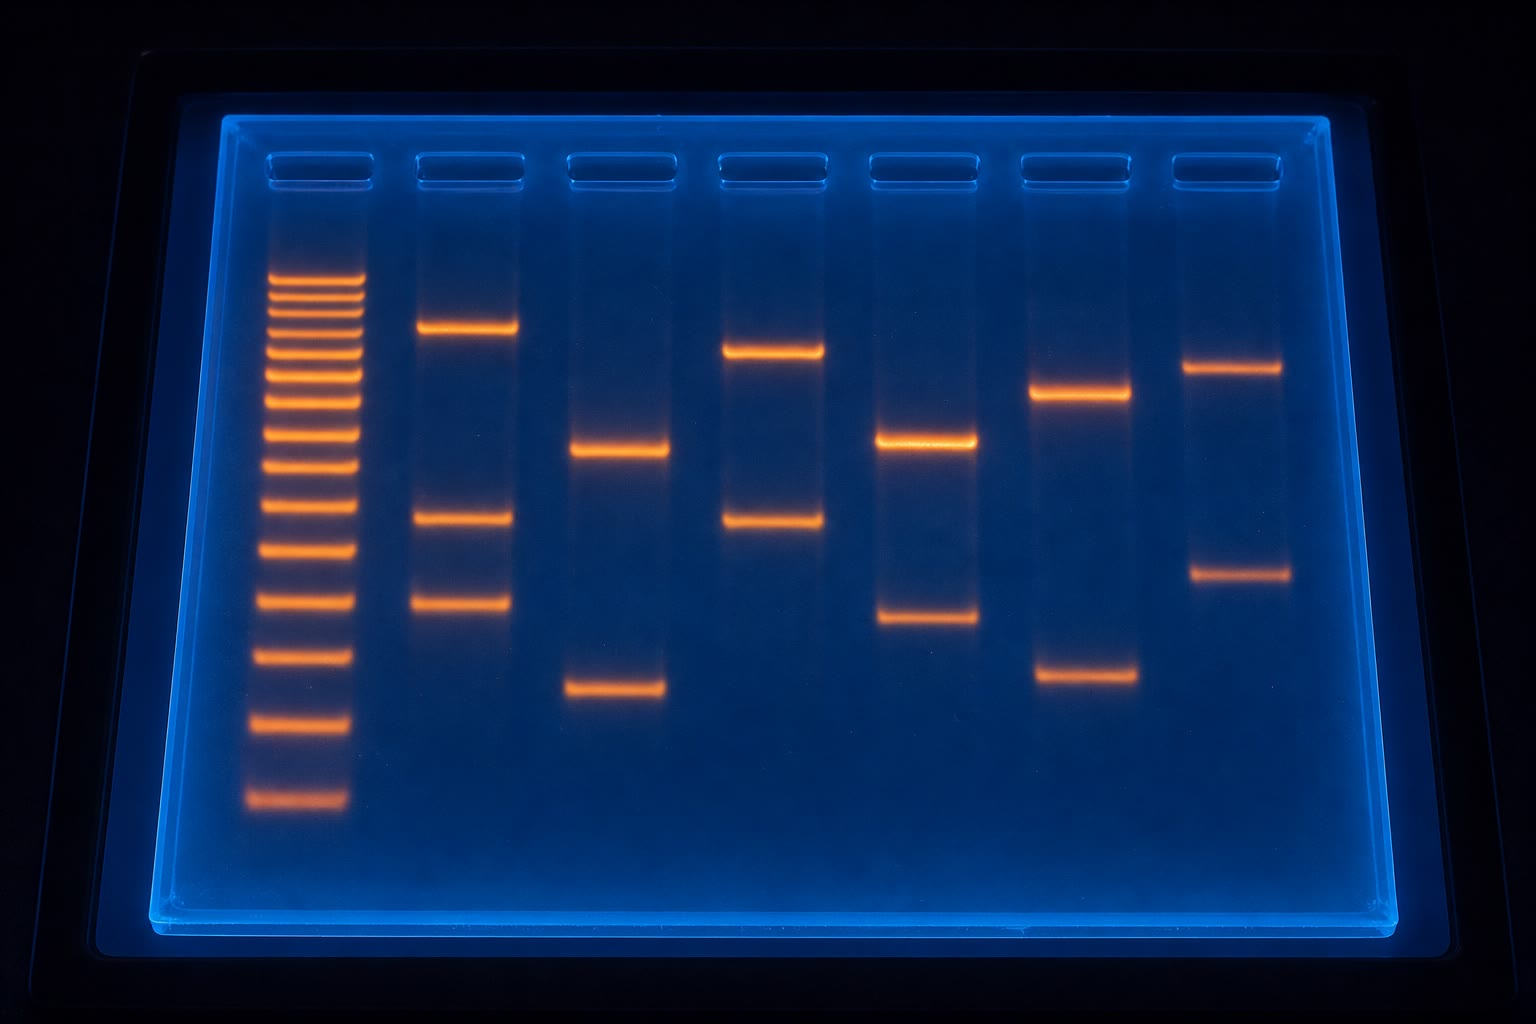
\includegraphics[width=0.56\linewidth]{images/book2/ai/g11-disease-gel.jpg}

{\small 紫外线下的凝胶电泳图：经荧光染色的 \omterm{def:g10:universal-dna:information}{DNA} 片段，
按长度分开。每一泳道为一个样本；
条带的排列模式即可读出\omterm{def:g10:universal-dna:gene}{等位基因}。}
\end{omfigure}

\begin{example}[检测能说明什么、不能说明什么]\label{ex:g11:genes-and-disease:testsays}
囊性纤维化的携带者检测，检查最常见的五十种\omterm{def:g11:mutations:mutation}{突变}\omterm{def:g10:universal-dna:gene}{等位基因}，
并可查出约 90\% 的携带者：阴性结果
可使一个人成为携带者的概率由 $1/25$ 降至约
$1/250$，但并不等于零。对两位已知携带者所生的胎儿作产前诊断，
结果几乎确定，并使父母面对
一个生物学无法替他们作出的决定。亨廷顿病的检测，
可告诉一位健康的三十岁者，其是否会患病；
三分之一有权知情者选择不知道。
\end{example}

\section{多基因疾病与生活方式}

\begin{proposition}[多因素疾病]\label{prop:g11:genes-and-disease:multifactorial}
最常见的疾病——包括 2 型糖尿病、心脏与动脉疾病、
多数癌症和哮喘——均为\emph{多因素疾病}\index{多因素疾病}：
数十乃至数百个\omterm{def:g10:universal-dna:gene}{等位基因}各自只使风险略微改变，而
环境（饮食、活动、吸烟、感染）则使风险大幅改变。
这类疾病在家族中出现，却不遵循
单\omterm{def:g10:universal-dna:gene}{基因}的规律；遗传易感性是一种风险，而非判决：
同样的\omterm{def:g10:universal-dna:gene}{等位基因}，在一种生活方式下导致发病，
在另一种生活方式下则不会。
\end{proposition}
\begin{proof}[证据]
同卵双胞胎共享全部\omterm{def:g10:universal-dna:gene}{等位基因}；若其中一人患 2 型
糖尿病，另一人约在 70\% 的情况下也患病——远高于
人群中的 8\%，可见\omterm{def:g10:universal-dna:gene}{基因}有影响——但并非 100\%，因此\omterm{def:g10:universal-dna:gene}{基因}并不
决定一切。人群在一代之内从农村饮食转为
城市饮食，患病率在\omterm{def:g10:universal-dna:gene}{基因}相同时升高了数倍。
在携带多个风险\omterm{def:g10:universal-dna:gene}{等位基因}的人中，坚持运动且
身材精瘦者，其患病率仅为不这样做者的
一小部分。
\end{proof}

\begin{omfigure}
\begin{tikzpicture}
\begin{axis}[
  ybar, bar width=12pt,
  width=0.8\linewidth, height=5.4cm,
  axis x line=bottom, axis y line=left,
  ymin=0, ymax=40, ylabel={60 岁前 2 型糖尿病患病率（\%）},
  ylabel style={font=\small},
  symbolic x coords={few risk alleles, average, many risk alleles},
  xtick=data, xticklabels={风险等位基因少, 平均, 风险等位基因多}, tick label style={font=\small},
  enlarge x limits=0.25, ytick={0,10,20,30,40},
  legend style={at={(0.5,-0.2)}, anchor=north, legend columns=2, font=\small, draw=none},
  nodes near coords, nodes near coords style={font=\scriptsize},
]
\addplot[fill=omMeth!50, draw=omMeth] coordinates {(few risk alleles,3) (average,6) (many risk alleles,12)};
\addplot[fill=omThm!50, draw=omThm] coordinates {(few risk alleles,9) (average,17) (many risk alleles,34)};
\legend{活动且偏瘦, 久坐且超重}
\end{axis}
\end{tikzpicture}

{\small 2 型糖尿病风险，按遗传评分与生活方式划分
（取自人群研究，经取整）。\omterm{def:g10:universal-dna:gene}{基因}使风险在评分两端相差
四倍；生活方式则使风险在每一评分点上都
扩大为三倍。两者共同作用。}
\end{omfigure}

\begin{remark}[那么，“遗传”究竟指什么]\label{rem:g11:genes-and-disease:meaning}
囊性纤维化在严格意义上是\omterm{def:g11:genes-and-disease:genetic}{遗传病}：\omterm{def:g11:enzymes-and-phenotype:phenotype}{基因型}
决定疾病，无论环境如何；环境
只改变病人的生活状况。2 型糖尿病在较弱的意义上是遗传的：
\omterm{def:g11:enzymes-and-phenotype:phenotype}{基因型}设定了一种易感性，环境
是否使之显现取决于环境。介于二者之间的是苯丙酮尿症，饮食
可抵消\omterm{def:g11:enzymes-and-phenotype:phenotype}{基因型}的效应，还有镰状\omterm{def:g10:cells-common-unit:cell}{细胞}贫血的携带者，其
\omterm{def:g10:universal-dna:gene}{等位基因}在一地是致病因素，在另一地却起保护作用。“它是否遗传？”
往往不是非此即彼的问题；真正该问的是：“程度多大，
在何种条件下？”才是应当追问的问题。
\end{remark}

\section{练习}

\begin{exercise}[$\star$]\label{exo:g11:genes-and-disease:1}
定义\omterm{def:g11:genes-and-disease:genetic}{隐性}\omterm{def:g10:universal-dna:gene}{等位基因}、\omterm{def:g11:genes-and-disease:genetic}{显性}\omterm{def:g10:universal-dna:gene}{等位基因}以及携带者。
\end{exercise}

\begin{exercise}[$\star$]\label{exo:g11:genes-and-disease:2}
囊性纤维化的两位携带者生育了一个孩子。求该孩子
患病、为携带者或两者都不是的概率。
\end{exercise}

\begin{exercise}[$\star$]\label{exo:g11:genes-and-disease:3}
根据\omterm{def:g11:genes-and-disease:pedigree}{系谱图}，写出 I-1、I-2、II-2 和
III-2 的\omterm{def:g11:enzymes-and-phenotype:phenotype}{基因型}。
\end{exercise}

\begin{exercise}[$\star$]\label{exo:g11:genes-and-disease:4}
为什么 X 连锁\omterm{def:g11:genes-and-disease:genetic}{隐性}\omterm{def:g11:genes-and-disease:genetic}{遗传病}在男性中远比在女性中常见？
\end{exercise}

\begin{exercise}[$\star$]\label{exo:g11:genes-and-disease:5}
什么是\omterm{prop:g11:genes-and-disease:multifactorial}{多因素疾病}？举出两个例子。
\end{exercise}

\begin{exercise}[$\star\star$]\label{exo:g11:genes-and-disease:6}
一位囊性纤维化患者与一位非携带者结婚。他们的
子女的情况如何？若其中某个子女为携带者，其子女又如何？
\end{exercise}

\begin{exercise}[$\star\star$]\label{exo:g11:genes-and-disease:7}
根据\omterm{def:g11:genes-and-disease:pedigree}{系谱图}，求 II-1 为
携带者的概率，以及 II-1 与一名来自
普通人群的男子所生子女患病的概率。
\end{exercise}

\begin{exercise}[$\star\star$]\label{exo:g11:genes-and-disease:8}
一名患亨廷顿病（\omterm{def:g11:genes-and-disease:genetic}{显性}，一个\omterm{def:g11:mutations:mutation}{突变}\omterm{def:g10:universal-dna:gene}{等位基因}）的男子与一名健康女子
育有四个子女。某个孩子遗传该病的概率是多少？
四个子女中无一人遗传该病的概率是多少？
\end{exercise}

\begin{exercise}[$\star\star$]\label{exo:g11:genes-and-disease:9}
一名血友病男子与一名非携带者女子结婚。描述他们
子女的\omterm{def:g11:enzymes-and-phenotype:phenotype}{基因型}和\omterm{def:g11:enzymes-and-phenotype:phenotype}{表型}，以及通过女儿与一名健康男子结婚所生的
孙辈的\omterm{def:g11:enzymes-and-phenotype:phenotype}{基因型}和\omterm{def:g11:enzymes-and-phenotype:phenotype}{表型}。
\end{exercise}

\begin{exercise}[$\star\star$]\label{exo:g11:genes-and-disease:10}
在凝胶图中，若某人携带两个
不同的\omterm{def:g11:mutations:mutation}{突变}\omterm{def:g10:universal-dna:gene}{等位基因}，其一增加了切割位点，另一个使
400 碱基对的片段再缺失 100 个碱基对，此人会出现哪些条带？
\end{exercise}

\begin{exercise}[$\star\star$]\label{exo:g11:genes-and-disease:11}
解释为什么囊性纤维化在欧洲的发病率
约为东亚的一千倍，而两地的\omterm{def:g11:mutations:mutation}{突变}率相同。
\end{exercise}

\begin{exercise}[$\star\star\star$]\label{exo:g11:genes-and-disease:12}
一对夫妇的第一个孩子患有囊性纤维化。计算第二个孩子患病的概率，
再计算接下来两个孩子中至少有一个患病的概率。
解释为什么“我们已经有了四分之一的概率”这一说法是谬误。
\end{exercise}

\begin{exercise}[$\star\star\star$]\label{exo:g11:genes-and-disease:13}
携带者检测能检出 90\% 的\omterm{def:g11:mutations:mutation}{突变}\omterm{def:g10:universal-dna:gene}{等位基因}。一名来自
普通人群的女子检测结果为阴性。计算她仍为携带者的概率，
以及她与一名已知为携带者的伴侣
所生子女患病的风险。
\end{exercise}

\begin{exercise}[$\star\star\star$]\label{exo:g11:genes-and-disease:14}
根据糖尿病图，对携带许多风险\omterm{def:g10:universal-dna:gene}{等位基因}的人，比较从“多”
到“少”风险\omterm{def:g10:universal-dna:gene}{等位基因}（不可能）与从久坐到活动（可能）的改变
所带来的效果。遗传风险评分应当用于
何种场合？
\end{exercise}

\begin{exercise}[$\star\star\star$]\label{exo:g11:genes-and-disease:15}
用一段文字讨论，亨廷顿病检测能为父母一方患病的健康青年
带来什么益处、付出什么代价，以及为什么这一决定
应由其本人做出。
\end{exercise}

\section{问题：一个家庭，一个基因}

\begin{problem}[{周末问题——一个囊性纤维化家庭
的三代追踪：确定基因型，计算每个计划中子女的患病风险，
读取一次实验室检测结果，并计算一个携带者群体中的
概率运算}]
\label{pb:g11:genes-and-disease:1}
莱娅和汤姆均健康，育有三个孩子：麦克斯（健康）、佐伊
（囊性纤维化）和卢（健康）。汤姆的妹妹安娜健康，
她与卡里姆结婚，卡里姆家族中无此病史；他们即将迎来
一个孩子。在人群中，每 25 人中有 1 人为携带者。

\medskip
\noindent\textbf{第一部分——\omterm{def:g11:enzymes-and-phenotype:phenotype}{基因型}。}
\begin{enumerate}
  \item 该病是\omterm{def:g11:genes-and-disease:genetic}{显性}还是\omterm{def:g11:genes-and-disease:genetic}{隐性}？请根据家系加以论证。
  \item 写出莱娅、汤姆和佐伊的\omterm{def:g11:enzymes-and-phenotype:phenotype}{基因型}。
  \item 麦克斯可能的\omterm{def:g11:enzymes-and-phenotype:phenotype}{基因型}有哪些，
        各自的概率是多少？
  \item 安娜为携带者的概率是多少？（考虑她的
        父母。）
  \item 卡里姆为携带者的概率是多少？
\end{enumerate}

\medskip
\noindent\textbf{第二部分——风险。}
\begin{enumerate}[resume]
  \item 计算安娜与卡里姆的孩子
        患病的概率。
  \item 莱娅和汤姆考虑生育第四个孩子，
        该孩子患病的概率是多少？为携带者的概率又是多少？
  \item 麦克斯成年后与一名来自普通人群的女子结婚，
        其第一个孩子患病的概率是多少？
  \item 佐伊成年后与一名来自普通人群的男子结婚，
        其子女患病的概率是多少？为携带者的概率是多少？
  \item 卢与一位表亲结婚，该表亲是安娜与卡里姆的孩子，
        计算其子女患病的概率。为什么这一概率高于
        麦克斯的情况？
\end{enumerate}

\medskip
\noindent\textbf{第三部分——检测。}
该家族所携带的\omterm{def:g11:mutations:mutation}{突变}\omterm{def:g10:universal-dna:gene}{等位基因}增加了一个切割位点：正常\omterm{def:g10:universal-dna:gene}{等位基因}
产生一个 900 碱基对的片段，\omterm{def:g11:mutations:mutation}{突变}\omterm{def:g10:universal-dna:gene}{等位基因}产生 600
和 300 碱基对的两个片段。
\begin{enumerate}[resume]
  \item 画出或描述佐伊、汤姆以及
        一名非携带者预期出现的条带。
  \item 对麦克斯进行检测：仅出现 900 碱基对的一条条带。他现在的\omterm{def:g11:enzymes-and-phenotype:phenotype}{基因型}是什么？
        结合第 8 题，重新计算其第一个孩子的风险。
  \item 对安娜进行检测：出现 900、600 和 300 碱基对的条带。重新计算
        其孩子的风险。
  \item 卡里姆的检测未发现人群中最常见的 50 种\omterm{def:g11:mutations:mutation}{突变}\omterm{def:g10:universal-dna:gene}{等位基因}，
        这些\omterm{def:g10:universal-dna:gene}{等位基因}覆盖了 90\% 的携带者。计算他仍为携带者
        的概率，并重新计算风险。
  \item 对安娜与卡里姆的胎儿进行产前检测，出现 900、
        600 和 300 碱基对的条带。该胎儿的\omterm{def:g11:enzymes-and-phenotype:phenotype}{基因型}和\omterm{def:g11:enzymes-and-phenotype:phenotype}{表型}是什么？
\end{enumerate}

\medskip
\noindent\textbf{第四部分——种群。}
\begin{enumerate}[resume]
  \item 若每 25 人中有 1 人为携带者，则随机一对夫妇
        双方均为携带者的概率是多少？由此
        推出患病新生儿的频率。
  \item 与观测值（每 2500 人中有 1 人）相比较，并加以评论。
  \item 过去几乎所有患者都在童年期死亡。试解释
        为什么\omterm{def:g11:mutations:mutation}{突变}\omterm{def:g10:universal-dna:gene}{等位基因}仍能保持在
        每 50 个拷贝中有 1 个的频率，
        并利用健康携带者与患者各自所携带的拷贝数加以说明。
  \item 如今的治疗使大多数患者能活到成年
        并生育子女。预测该\omterm{def:g10:universal-dna:gene}{等位基因}频率在未来几代中的
        变化方向及其大小。
  \item 总结结论：两名携带者所生子女患病的四分之一概率，
        健康同胞为携带者的三分之二概率，以及凝胶结果
        为该家庭的计算增加了什么。
\end{enumerate}
\end{problem}
